\documentclass[border=2pt]{standalone}
\usepackage{pgfplots}
\pgfplotsset{compat=1.18}
\begin{document}
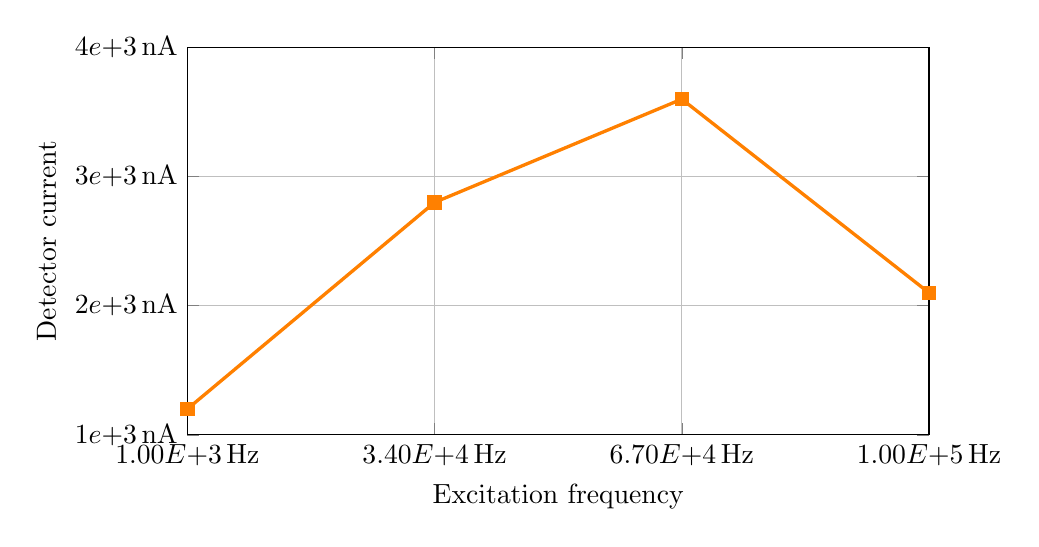
\begin{tikzpicture}
  \begin{axis}[
    width=11cm,
    height=6.5cm,
    xmin=1000,
    xmax=100000,
    ymin=1000,
    ymax=4000,
    xtick={1000,34000,67000,100000},
    ytick={1000,2000,3000,4000},
    scaled ticks=false,
    xticklabel={$\pgfmathprintnumber[sci,sci E,sci zerofill,precision=2]{\tick}\,\mathrm{Hz}$},
    yticklabel={$\pgfmathprintnumber[sci,sci e,sci precision=1]{\tick}\,\mathrm{nA}$},
    grid=major,
    xlabel={Excitation frequency},
    ylabel={Detector current}
  ]
    \addplot[orange,very thick,mark=square*] coordinates {
      (1000,1200) (34000,2800) (67000,3600) (100000,2100)
    };
  \end{axis}
\end{tikzpicture}
\end{document}
